%%%%%%%%%%%%%%%%%%%%%%%%%%%%%%%%%%%%%%%%%
%
% (c) 2019 by Jennifer Laaser
%
% This work is licensed under the Creative Commons Attribution-NonCommercial-ShareAlike 4.0 International License. To view a copy of this license, visit http://creativecommons.org/licenses/by-nc-sa/4.0/ or send a letter to Creative Commons, PO Box 1866, Mountain View, CA 94042, USA.
%
% The current source for these materials is accessible on Github: https://github.com/jlaaser/pogil-polymers
%
%%%%%%%%%%%%%%%%%%%%%%%%%%%%%%%%%%%%%%%%%

\renewcommand{\figpath}{content/polymphys/mechanical-properties/viscoelasticity/figs}
\newcommand{\labelbase}{}
\renewcommand{\labelbase}{viscoelasticity}

\begin{activity}[Viscoelasticity of Polymeric Materials]

\begin{instructornotes}

	This activity introduces students to ...
	
	After completing this activity, students will be able to:
			\begin{enumerate}
				\item ...
			\end{enumerate}
	
			
	\subsection*{Activity summary:}
	\begin{itemize}
		\item \textbf{Activity type:} Learning Cycle
		\item \textbf{Content goals:} ...
		\item \textbf{Process goals:} %https://pogil.org/uploads/attachments/cj54b5yts006cklx4hh758htf-process-skills-official-pogil-list-2015-original.pdf
			written communication, critical thinking, information processing
		\item \textbf{Duration:} TBD %approx. 45 minutes without class discussion
		\item \textbf{Instructor preparation required:} 
			\begin{itemize}
				\item Prepare small samples of silly putty (or comparable silicone putty) for each student group
			\end{itemize}
		\item \textbf{Related textbook chapters:}
			\begin{itemize}
				\item \emph{Polymer Chemistry} (Hiemenz \& Lodge): ...
			\end{itemize}
	\end{itemize}

\end{instructornotes}

	%\textbf{Focus question:} Put a central question for the students to consider through this exercise here.

\begin{model}[Properties of Silicone Putty]
\label{model:sillyputty}

	Obtain a small sample of silicone putty from your instructor.
	
	Do the following experiments, and note your observations about how the material responds:
	
	\begin{enumerate}
		\item Place a small ball of putty on a table, and hit it quickly with your hand.
			\begin{itemize}
				\item Observations:
				
				\begin{solution}[0.75in]
				
					The putty mostly retains its shape.
					
				\end{solution}
			\end{itemize}
		
		\item Place a small ball of putty on your desk, and let it sit without touching it for 1-2 minutes.
			\begin{itemize}
				\item Observations:
				
				\begin{solution}[0.75in]
				
					The putty initially retains its shape, but over time, slowly begins to flow and flatten out.
					
				\end{solution}
			\end{itemize}
		
		\item Take a small piece of putty and stretch it between your hands.  Vary the rate at which you stretch it (quickly vs. slowly).
			\begin{itemize}
				\item Observations:
				
				\begin{solution}[1in]
				
					When the putty is pulled slowly, it stretches like taffy.
					
					When the putty is pulled quickly, it may break.
					
				\end{solution}
			\end{itemize}
		
	\end{enumerate}

\end{model}


\begin{ctqs}

	\question In which of your experiments would you say the putty behaved more like an \emph{elastic solid}?  Briefly explain your reasoning.
	
		\begin{solution}[1.25in]
		
			In experiment (1), the putty retains its shape, and is thus more solid-like.
			
			In experiment (3), when pulled quickly, the putty ``breaks'', which is also a solid-like behavior.
		
		\end{solution}
	
	\question In which of your experiments would you say the putty behaved more like a \emph{viscous liquid}?  Briefly explain your reasoning.
	
		\begin{solution}[1in]
		
			In experiment (2), the putty flowed to match the shape of the surface it was sitting on, which is a liquid-like behavior.
		
		\end{solution}
	
	\question How did your observation of solid-like or liquid-like properties depend on the timescale on which you observed it?
	
		\begin{solution}[1in]
		
			On short timescales, the putty behaved more like a solid.
			
			On long timescales, the putty behaved more like a liquid.
			
		\end{solution}
		
	\question Explain, in one or two complete sentences, why you think we might describe this putty as a ``viscoelastic'' material.
	
			\begin{solution}[1.5in]
			
				We describe this putty as a viscoelastic material because it  has some properties of both elastic solids (elasticity, ability to hold its shape) and of viscous liquids (ability to flow).  The properties that we observe depend on the timescale of the observation.
				
			\end{solution}
		
\end{ctqs}

\begin{model}[The Stress Response of Solids]

	explain a step-strain experiment for a spring
	
\end{model}

\begin{ctqs}
	\question WALK STUDENTS THROUGH ELASTIC SOLID (BY ANALOGY TO RUBBER BAND)
	
\end{ctqs}

\begin{infobox}

	Solid-like materials are typically described in terms of their \emph{modulus}, E (for extensional strain) or G (for shear strain).  For an elastic solid subjected to a strain of size $\epsilon$ (for extensional strain) or $\gamma$ (for shear strain), the resulting stress, $\sigma$, is directly proportional to the strain:
	\begin{align*}
		\sigma &= E\epsilon\,\,\,\,\,\,\,\text{(extensional strain)}\\
		%&\text{or}\\
		\text{or}\,\,\,\,\,\,\sigma &= G\gamma\,\,\,\,\,\,\,\text{(shear strain)}
	\end{align*}
	
\end{infobox}

\begin{ctqs}
	\question PLOT STRESS PROFILES FOR STEP-STRAIN
	
	\question ARE THEY CONSISTENT WITH PREDICTIONS?
\end{ctqs}

\begin{model}[The Stress Response of Liquids]

	explain a step-strain experiment for a viscous liquid
	
\end{model}

\begin{ctqs}
	
	\question  WALK STUDENTS THROUGH VISCOUS LIQUID (BY ANALOGY TO MOVING HAND THROUGH WATER)
	
\end{ctqs}

\begin{infobox}
	
	Liquid-like materials are typically described in terms of their \emph{viscosity}, $\eta$.  For a liquid, the stress is proportional to the strain \emph{rate}:
	\begin{align*}
		\sigma &= \eta\frac{d\epsilon}{dt}=\eta\dot\epsilon\,\,\,\,\,\,\,\text{(extensional strain)}\\
		%&\text{or}\\
		\text{or}\,\,\,\,\,\,\sigma &= \eta\frac{d\gamma}{dt}=\eta\dot\gamma\,\,\,\,\,\,\,\text{(shear strain)}
	\end{align*}

\end{infobox}

\begin{ctqs}
	\question PLOT STRESS PROFILES FOR STEP-STRAIN
	
	\question ARE THEY CONSISTENT WITH PREDICTIONS?
\end{ctqs}
	

\begin{model}[The Maxwell Model]
\label{\labelbase:mdl:maxwell}

	One simple way to describe the viscoelasticity of polymeric materials is to imagine the response of the material as being represented by a spring \emph{and} a dashpot, connected in series
	
	\centerline{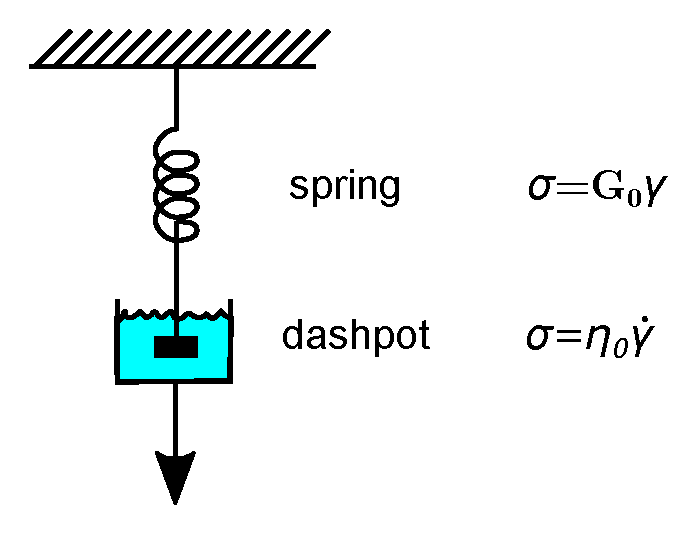
\includegraphics[width=0.5\textwidth]{\figpath/model2-maxwellelement}}
	
	This model is called the \emph{Maxwell Model}; in this model, the spring represents the elastic solid-like portion of the material's response, while the dashpot represents the viscous liquid-like portion of the material's response.
	
\end{model}

	
\begin{ctqs}
	\question (GET THEM TO REASON THROUGH EXPONENTIAL DECAY)
	
					\begin{solution}[2.5in]
					\end{solution}
					
\end{ctqs}

\begin{infobox}
	As shown in Exercise \ref{\labelbase:exc:maxwell}, the time-dependent stress for a step-strain experiment on the Maxwell model works out to be:
	\begin{align*}
		\sigma(t) = \sigma_0 e^{-t G_0/\eta_0}  && \text{or} && \sigma(t) = \sigma_0 e^{-t /\tau}
	\end{align*}
	where $\tau = \eta_0/G_0$.
\end{infobox}

\begin{ctqs}
	
	\question Is this equation consistent with your prediction from question  NNN?  Why or why not?
	
					\begin{solution}[1.5in]
					\end{solution}
		
	\question At what time $t$ will $\sigma(t)$ drop to 1/e of its initial value?
	
					\begin{solution}[1.5in]
					\end{solution}
		
		\question Why might we refer to $\tau$ as the ``characteristic relaxation timescale''?  Explain your reasoning in 1-2 complete sentences.
	
					\begin{solution}[1.5in]
					\end{solution}
					
		\question The silicone putty that you investigated at the beginning of this activity has a characteristic relaxation timescale of approximately 10 minutes.
		
			\begin{enumerate}
				\item On timescales \emph{shorter} than this characteristic relaxation time, did the putty appear to be more liquid-like or more solid-like?
	
					\begin{solution}[0.75in]
					
						The putty appeared to be more solid-like on short observation timescales.
						
					\end{solution}
				
				\item On timescales \emph{longer} than this characteristic relaxation time, did the putty appear to be more liquid-like or more solid-like?
	
					\begin{solution}[0.75in]
					
						The putty appeared to be more liquid-like over long observation timescales.
						
					\end{solution}
				
				\item In three or four complete sentences, briefly summarize the relationship between the characteristic relaxation time, the timescale of your observation, and the perceived liquid-like or solid-like properties of the material.
	
					\begin{solution}[2.5in]
					\end{solution}
			\end{enumerate}
		
\end{ctqs}
	

%\clearpage
\begin{exercises}

		\exercise Viscoelastic properties can arise from a number of molecular-scale interactions.  Which of the following do you think would give rise to viscoelastic properties in a polymeric material?  For each interaction that you think would cause a viscoelastic response, identify the physical process that you think would be most closely associated with the relaxation time of the material.
		
			\begin{enumerate}
				\item Covalent crosslinking of the polymer chains
				\item Hydrogen bonds (or other ``sticky'' noncovalent interactions) between polymer chains
				\item ``Tangling'' of long polymer chains around each other
			\end{enumerate}
			
		% exercise connecting to polymer processing? e.g. why is it important to control viscoelasticity in processing?
		
		\exercise In our discussion of the Maxwell Model, we considered a step-strain experiment, where we pulled the material to a set distance and then held it there.
		
			Another type of experiment we could conduct is a ``step-stress'' experiment, in which we simply begin pulling on the material with a constant force.  Make plots of (a) the applied stress and (b) the resulting strain that you would expect for this experiment.
			
		\exercise \label{\labelbase:exc:maxwell} DERIVE STEP-STRESS RESPONSE FOR MAXWELL MODEL
		
		\exercise The Maxwell Model is one simple model that yields viscoelastic behavior.  Another model that gives viscoelastic behavior is the Voigt model, in which the spring and dashpot are connected in parallel rather than in series:
		
			\centerline{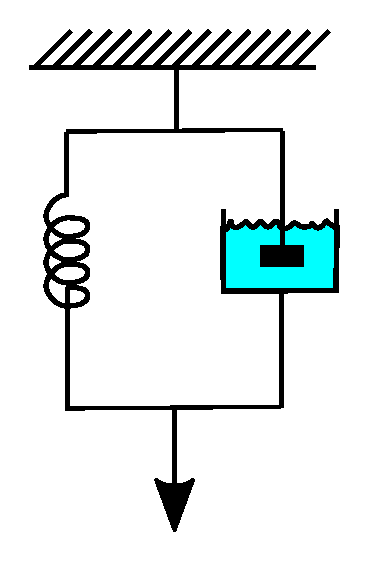
\includegraphics[width=0.25\textwidth]{\figpath/exercises-voigtelement}}
			
			In this case, the total \emph{stress} is the sum of the stresses across the two components, while the total \emph{strain} is identical for each component.
			
			\begin{enumerate}
				\item Express the above statement using appropriate mathematical equations.  Then, find an expression for the total stress in terms of $G_0$, $\eta_0$, and $\gamma$.
				\item Qualitatively, how would you expect the Voigt element to respond to (a) a step strain experiment, and (b) a step stress experiment?  Plot the expected response for each case.
				%\item Find a functional form for the strain, $\gamma(t)$, that results from a step stress of magnitude $\sigma_0$ (note: this is challenging, and requires some knowledge of differential equations).
					%Note: should coach this one more!
			\end{enumerate}
		
\end{exercises}
	
\end{activity}